%\section{Techniques of measuring vasomotion} 
\label{freq}

For some time it has been the interest of researchers and health care clinicians to get a better understanding of the mechanisms that control and regulate local blood flow in the microcirculatory system\cite{sagaidachnyi2014,sagaidachnyi2017,geyer2004,liu2012}. 
Visualization of the vessels in skin and the way these behave can be important for assessment of stages of sepsis as mentioned before in \cref{chap:sepsis}, but also in peripheral vascular disease, the results of skin reconstructive surgery, wound and ulcer management.\cite{liu2012,kanta2014}
Spectral components of vasomotion seem to vary when influenced of some diseases. An example could be a decrease in amplitude of endothelial blood flow oscillations is assumed to be a biomaker for endothelial dysfunction. Endothelial dysfunction indicate cardiovascular disorders such as arterial hypertension and cardiac ischemia. An increased amplitude within the neurogenic frequency band is characterized by a decrease of vascular resistance and an increase of blood flow through the arteriovenous shunt.\cite{sagaidachnyi2017}

For measuring regulation in the peripheral blood flow, it is assumed that these oscillating changes are the source of thermal waves propagating from microvessels toward the skin surface. Especially thermal imaging uses this concept.\cite{sagaidachnyi2017}
Furthermore a correlation between skin temperature in fingertips and blood flow oscillations has been found\cite{sagaidachnyi2014}.
When the thermal waves propagate from the vessels towards the skin surface they are prone to some attenuation. This is due to skin properties that function like a low-frequency filter.\cite{podtaev2008}
The magnitude of attenuation is directly proportional to the frequency and the frequency depends on the velocity of the wave propagation \cite{sagaidachnyi2014}.
Therefore as illustrated in \cref{fig:atten}, a higher frequency leads to a higher attenuation.   

\begin{figure}[H]
	\centering	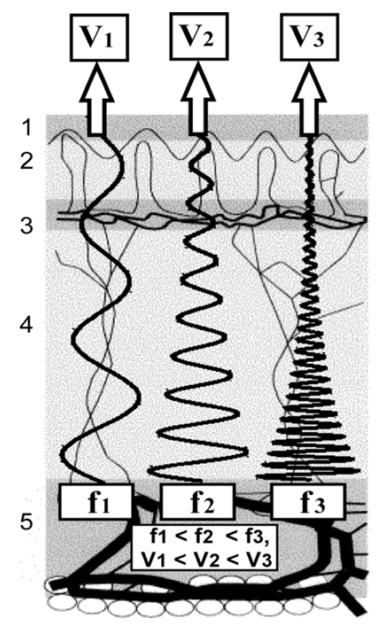
\includegraphics[width=0.28\textwidth]{figures/attenuation}
	\caption{Graphical representation of amplitude dampening through the skin in three signals with different frequency $f_{1}$ - $f_{3}$ and velocity $V_{1}$ - $V_{3}$.\cite{sagaidachnyi2014}}
	\label{fig:atten}
\end{figure} \vspace{-.3cm}

There are multiple different techniques of measuring blood flow in the peripheral circulatory system. For example capillaroscopy, laser Doppler flowmetry (LDF), and thermal imaging. These have been used differently trying to quantify functional aspects of skin vasculature.\cite{liu2012} Laser Doppler flowmetry is one of the most used\cite{geyer2004} and thermal imaging being introduced as a new technique of measuring vasoregulation\cite{sagaidachnyi2014}.

\section{Thermal imaging}
\label{sec:thermalImaging}
In studies made by a Russian group by Sagaidachnyi et al. thermal imaging has been used to study vasomotion. In their studies they sought to get better understanding of the relationship between blood flow oscillations and temperature oscillations, and if it was possible to recreate the blood flow oscillation from temperature recording. Recordings of flow were done by Photoplethysmography and temperature of the skin by thermal imaging. The recordings were made on a small point of the fingertip. Trough their work, five frequency bands were identified as vasomotion activity, and are following: endothelial (0.005–0.02 Hz), neurogenic (0.02-0.05 Hz), myogenic (0.05-0.15 Hz), respiratory origin (0.15-0.4 Hz) and cardiac origin (0.4-2.0 Hz).\cite{sagaidachnyi2017,sagaidachnyi2014}
The choice of using thermal imaging to study vasomotion implies certain advantages. Mainly a larger sample area, but also a higher temporal, (up to 105 fps) and spatial (2048 × 1536 pixels) resolution. In addition it is also a non invasive way of measuring vasomotion.\cite{sagaidachnyi2017}

\section{Laser Doppler flowmetry}
In an other study from Geyer et al. vasomotion is investigated trough the use of laser Doppler flowmetry as recording technique. In the study vasoregulation variables are sought quantified. LDF is a non invasive approach to measuring changes in vasomotion. The technique register changes in the depth of 1 mm, and works like Doppler ultrasound, utilizing the shift in frequency. Though instead of using ultrasonic waves, LDF uses light reflected from red blood cells. This study found the same frequency bands as Sagaidachnyi et al. with minimal difference. Data obtained were analyzed trough spectral analysis. Wavelet transform was used instead of the most used fourier analysis, because wavelet analysis offered better resolution to reveal characteristics in the low frequency area.\cite{geyer2004}
LDF uses a small sample area and the laser probe allows a sampling area as small as 1 mm$^3$.\cite{brothers2010} 


  
\section{Summarizing}

Both Geyer et al. and Sagaidachnyi et al. managed to show spectral components relating to vasomotion. The techniques both uses an non invasive approach, even though the methods are different when measuring red blood cell count compared to temperature. The use of thermal imaging as the method of measuring vasomotion offers interesting opportunities. Larger sampling area would allow interpretation and study of a more global tissue area. Along with the resolution of thermal imaging cameras, this makes thermal imaging the choice of measuring technique to be used in this study. 



